\documentclass[10pt]{extarticle}

\usepackage[english]{babel}
\usepackage[T1]{fontenc}
\usepackage{lmodern,mathrsfs}
\usepackage{xparse}
\usepackage[inline,shortlabels]{enumitem}
\setlist{topsep=2pt,itemsep=2pt,parsep=0pt,partopsep=0pt}
\usepackage[dvipsnames]{xcolor}
\usepackage[utf8]{inputenc}
\usepackage[a4paper,top=0.5in,bottom=0.2in,left=0.5in,right=0.5in,footskip=0.3in,includefoot]{geometry}
\usepackage[most]{tcolorbox}
\tcbuselibrary{minted} % tcolorbox minted library, required to use the "minted" tcb listing engine (this library is not loaded by the option [most])
\usepackage{minted} % Allows input of raw code, such as Python code
\usepackage[colorlinks]{hyperref} % ALWAYS load this package LAST

\usepackage{graphicx}
\usepackage{fancyhdr}
\usepackage{float}

\geometry{top=2.5cm, bottom=2.5cm, left=2cm, right=2cm}

% Custom tcolorbox style for Python code (not the code or the box it appears in, just the options for the box)
\tcbset{
    pythoncodebox/.style={
        enhanced jigsaw,breakable,
        colback=gray!10,colframe=gray!20!black,
        boxrule=1pt,top=2pt,bottom=2pt,left=2pt,right=2pt,
        sharp corners,before skip=10pt,after skip=10pt,
        attach boxed title to top left,
        boxed title style={empty,
            top=0pt,bottom=0pt,left=2pt,right=2pt,
            interior code={\fill[fill=tcbcolframe] (frame.south west)
                --([yshift=-4pt]frame.north west)
                to[out=90,in=180] ([xshift=4pt]frame.north west)
                --([xshift=-8pt]frame.north east)
                to[out=0,in=180] ([xshift=16pt]frame.south east)
                --cycle;
            }
        },
        title={#1}, % Argument of pythoncodebox specifies the title
        fonttitle=\sffamily\bfseries
    },
    pythoncodebox/.default={}, % Default is No title
    %%% Starred version has no frame %%%
    pythoncodebox*/.style={
        enhanced jigsaw,breakable,
        colback=gray!10,coltitle=gray!20!black,colbacktitle=tcbcolback,
        frame hidden,
        top=2pt,bottom=2pt,left=2pt,right=2pt,
        sharp corners,before skip=10pt,after skip=10pt,
        attach boxed title to top text left={yshift=-1mm},
        boxed title style={empty,
            top=0pt,bottom=0pt,left=2pt,right=2pt,
            interior code={\fill[fill=tcbcolback] (interior.south west)
                --([yshift=-4pt]interior.north west)
                to[out=90,in=180] ([xshift=4pt]interior.north west)
                --([xshift=-8pt]interior.north east)
                to[out=0,in=180] ([xshift=16pt]interior.south east)
                --cycle;
            }
        },
        title={#1}, % Argument of pythoncodebox specifies the title
        fonttitle=\sffamily\bfseries
    },
    pythoncodebox*/.default={}, % Default is No title
}

% Custom tcolorbox for Python code (not the code itself, just the box it appears in)
\newtcolorbox{pythonbox}[1][]{pythoncodebox=#1}
\newtcolorbox{pythonbox*}[1][]{pythoncodebox*=#1} % Starred version has no frame

% Custom minted environment for Python code, NOT using tcolorbox
\newminted{python}{autogobble,breaklines,mathescape}

% Custom tcblisting environment for Python code, using the "minted" tcb listing engine
% Adapted from https://tex.stackexchange.com/a/402096
\NewTCBListing{python}{ !O{} !D(){} !G{} }{
    listing engine=minted,
    listing only,
    pythoncodebox={#1}, % First argument specifies the title (if any)
    minted language=python,
    minted options/.expanded={
        autogobble,breaklines,mathescape,
        #2 % Second argument, delimited by (), denotes options for the minted environment
    },
    #3 % Third argument, delimited by {}, denotes options for the tcolorbox
}

%%% Starred version has no frame %%%
\NewTCBListing{python*}{ !O{} !D(){} !G{} }{
    listing engine=minted,
    listing only,
    pythoncodebox*={#1}, % First argument specifies the title (if any)
    minted language=python,
    minted options/.expanded={
        autogobble,breaklines,mathescape,
        #2 % Second argument, delimited by (), denotes options for the minted environment
    },
    #3 % Third argument, delimited by {}, denotes options for the tcolorbox
}

% verbbox environment, for showing verbatim text next to code output (for package documentation and user learning purposes)
\NewTCBListing{verbbox}{ !O{} }{
    listing engine=minted,
    minted language=latex,
    boxrule=1pt,sidebyside,skin=bicolor,
    colback=gray!10,colbacklower=white,valign=center,
    top=2pt,bottom=2pt,left=2pt,right=2pt,
    #1
} % Last argument allows more tcolorbox options to be added

\setlength{\parindent}{0.2in}
\setlength{\parskip}{0pt}
\setlength{\columnseprule}{0pt}

\makeatletter
% Redefining the title block
\renewcommand\maketitle{
    \null\vspace{4mm}
    \begin{center}
        {\Huge\sffamily\bfseries\selectfont\@title}\\
            \vspace{4mm}
        {\Large\sffamily\selectfont\@author}\\
            \vspace{4mm}
        {\large\sffamily\selectfont\@date}
    \end{center}
    \vspace{6mm}
}
% Adapted from https://tex.stackexchange.com/questions/483953/how-to-add-new-macros-like-author-without-editing-latex-ltx?noredirect=1&lq=1
\makeatother

\pagestyle{fancy}
\fancyhead[L]{\textbf{Data Science with Python}}
\fancyhead[C]{}
\fancyhead[R]{January 2025}

\begin{document}

\begin{center}
    \textbf{\huge Data Visualization with Python} \\
    \vspace{0.5cm}
    \textit{Categorical Data Analysis using Catplot} \\
    \vspace{1cm}
    \textbf{Hernández Pérez Erick Fernando} \\
    \vspace{0.5cm}
\end{center}

\begin{python}[The simplest example](style=one-dark){colback=gray!40!black,colframe=blue}
import seaborn as sns

df = sns.load_dataset("titanic")
sns.catplot(data=df, x="age", y="class")
\end{python}

\noindent Carplot is a function within the Seaborn library. We can say that its functionality lies in showing the relationship between a numerical variable (that which represents quantities, being continuous and discrete) and one or more categorical variables (that which represents categories or groups, their values are qualitative and can be divided into nominal and ordinal), providing us with multiple possible representations for this purpose.

\begin{figure}[h!]
    \centering
    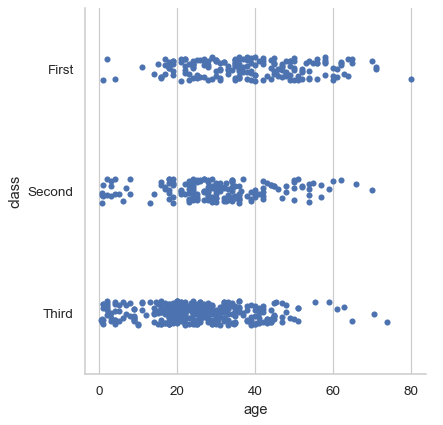
\includegraphics[width=0.5\textwidth]{img/catplot_1_0.png} 
    \caption{The simplest example}
    \label{fig:imagen}
\end{figure}

In the simplest example we can see that our numerical variable is age (values with a minimum of 0.42 and a maximum of 80, although they can be easily discretized by rounding down), while the categorical variable is class (first, second and third class).

From this graph we can obtain information in a very simple way. We can conclude that in the third class there were many people between a little before 20 years old and 40 years old; this being the class with the highest density. The second class is also centered on the 20-40 interval but is clearly more distributed across age ranges. Finally, the first class is the class that seems to be most evenly distributed between the 20-60 range, as is the class with the maximum age of 80 years.

Similarly, this example shows that the default visual representation is a jittered strip plot. But, obviously, we are not limited to this as we will see later.

\section{Parameters}


\noindent Before looking at other application examples, let's analyze the most important parameters that will allow us to start using catplot in our analysis.

\begin{itemize}
    \item \textbf{data}: It is the dataset where Seaborn will look for the variables that you indicate. It can be a Pandas DataFrame, a list, a dictionary, an array, etc.
    \item \textbf{x}: The variable that will go on the X-axis.
    \item \textbf{y}: The variable that will go on the Y-axis.
    \item \textbf{hue}: This parameter allows you to specify a categorical variable that will be used to differentiate the data by color. The color of the dots or bars will change according to the values of the variable specified in hue. You can see how to plot a third dimension (Graph of complex variable functions for example).
    \item \textbf{row, col}:
    These are categorical variables that are used to divide the data into subgraphs (facets) and create a “grid” of graphs. Each combination of row and col values generates a different graph on a grid.
    \item \textbf{kind}: Define the type of chart you want to create. This parameter indicates what type of visualization you are going to use for your categorical data.
    \begin{enumerate}
        \item "strip": A plot of points (one for each observation), scattered along the X-axis.
        \item “swarm": Similar to the strip, but the points are arranged to avoid overlapping.
        “box": A box plot showing the median, quartiles and outliers.
        \item “violin": Combines a box plot with a density distribution, similar to a violin.
        \item “boxen": An advanced variant of the box plot that shows more details of the distribution.
        \item “point": A dot plot representing averages and standard errors, useful for comparing categories.
        \item “bar": A bar chart showing the mean or quantity of each category.
        \item “count: A bar chart showing the number of items in each category.
    \end{enumerate}
    \item \textbf{legend}: Controls how the legend (the part of the chart that explains the meaning of the mark colors or styles) is drawn. You have several options.
    \begin{enumerate}
        \item "auto": The legend will automatically adjust between a brief or full representation depending on the number of levels (categories) in hue or size.
        \item "brief": The legend will show only a sample of evenly spaced values, useful when you have many categories or levels in hue or size.
        \item "full": Each group or category will have a full entry in the legend, even if there are many categories.
        \item False: No legend is drawn, even if hue or size is used.
    \end{enumerate}
\end{itemize}

And that's it, of course there are other parameters that were left out, but these should be enough for you to try your own graphs with catplot.

Before continuing, we will see how the type of graph can give us more or less information.

Compare the analysis given for the simplest example and, as an exercise, complete it with your own analysis.

\begin{python}[The simplest example with 'boxen'](style=one-dark){colback=gray!40!black,colframe=blue}
sns.catplot(data=df, x="age", y="class", kind='boxen')
\end{python}

\begin{figure}[h!]
    \centering
    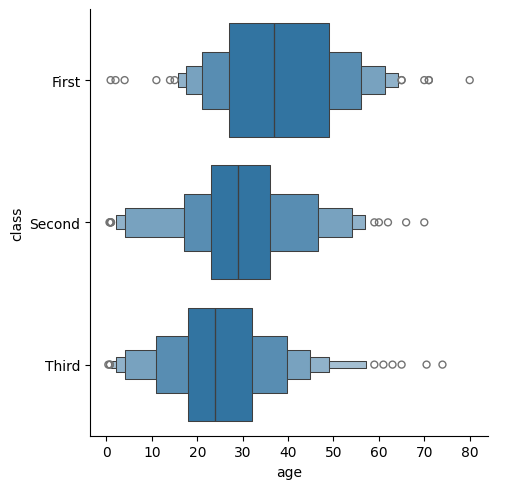
\includegraphics[width=0.5\textwidth]{img/catplot_2.png} 
    \caption{The simplest example but with 'boxen}
    \label{fig:imagen}
\end{figure}

\newpage

\section{Applied cases}

We will consider the dataset Seaborn has 'tips', which is a dataset containing information about tips given in a restaurant. The reason for this choice is that it has several categorical variables.

\begin{python}[tips](style=one-dark){colback=gray!40!black,colframe=blue}
import matplotlib.pyplot as plt
import pandas as pd
import seaborn as sns
from sklearn.preprocessing import LabelEncoder

tips = sns.load_dataset("tips")
tips.info()
\end{python}

\begin{figure}[H]
    \centering
    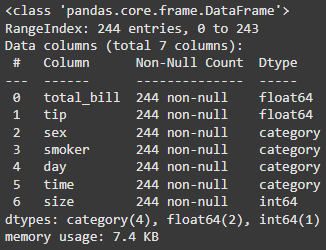
\includegraphics[width=0.5\textwidth]{img/info_tips.png} 
    \caption{tips.info()}
    \label{fig:imagen}
\end{figure}

\begin{python}[tips](style=one-dark){colback=gray!40!black,colframe=blue}
sns.catplot(data=tips, x='day', y='tip', hue='sex', kind='violin')
\end{python}

\begin{figure}[H]
    \centering
    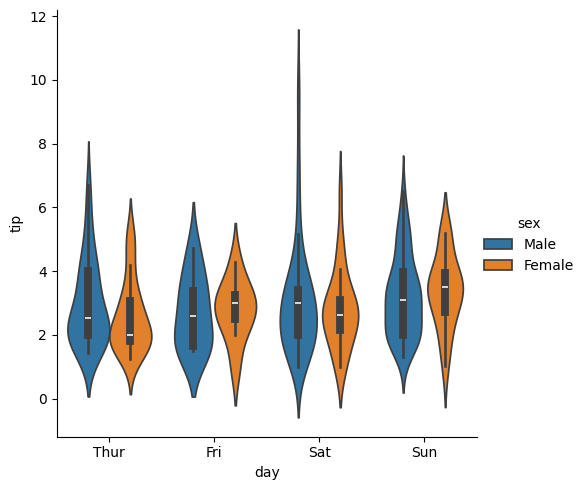
\includegraphics[width=0.5\textwidth]{img/catplot_3.png} 
    \caption{Tips given by each sex on each day}
    \label{fig:imagen}
\end{figure}

\begin{python}[tips](style=one-dark){colback=gray!40!black,colframe=blue}
sns.catplot(data=tips, x='day', y='total_bill', hue='sex', kind='violin')
\end{python}

\begin{figure}[H]
    \centering
    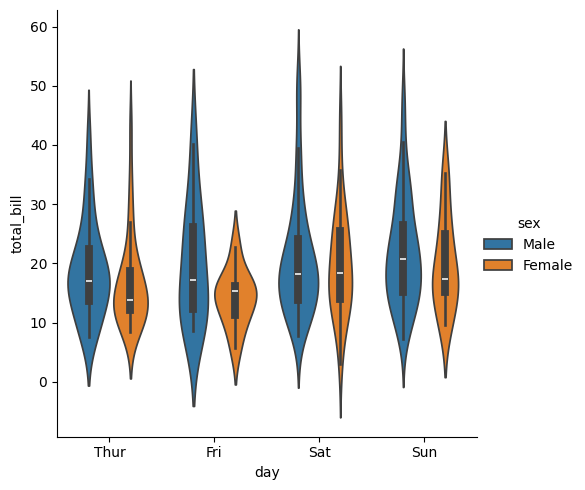
\includegraphics[width=0.5\textwidth]{img/catplot_4.png} 
    \caption{Total bill for each day depending on sex}
    \label{fig:imagen}
\end{figure}

\begin{python}[tips](style=one-dark){colback=gray!40!black,colframe=blue}
encoder = LabelEncoder()

tips['sex'] = encoder.fit_transform(tips['sex']) # 0-F 1-M
tips['smoker'] = encoder.fit_transform(tips['smoker'])
tips['time'] = encoder.fit_transform(tips['time']) # 0-D 1-L
day_mapping = {'Thur': 1, 'Fri': 2, 'Sat': 3, 'Sun': 4}
tips['day'] = tips['day'].map(day_mapping)

df_melt = pd.melt(tips, id_vars=['time'], value_vars=['smoker', 'sex'])
df_melt = df_melt.groupby(['time', 'variable'])['value'].value_counts().to_frame()

g = sns.catplot(df_melt, x='variable', y='count', hue='value',
                col='time',kind='bar')

new_labels = ["[Female, No]", "[Male, Yes]"]
for t, l in zip(g._legend.texts, new_labels):
    t.set_text(l)
\end{python}

\begin{figure}[H]
    \centering
    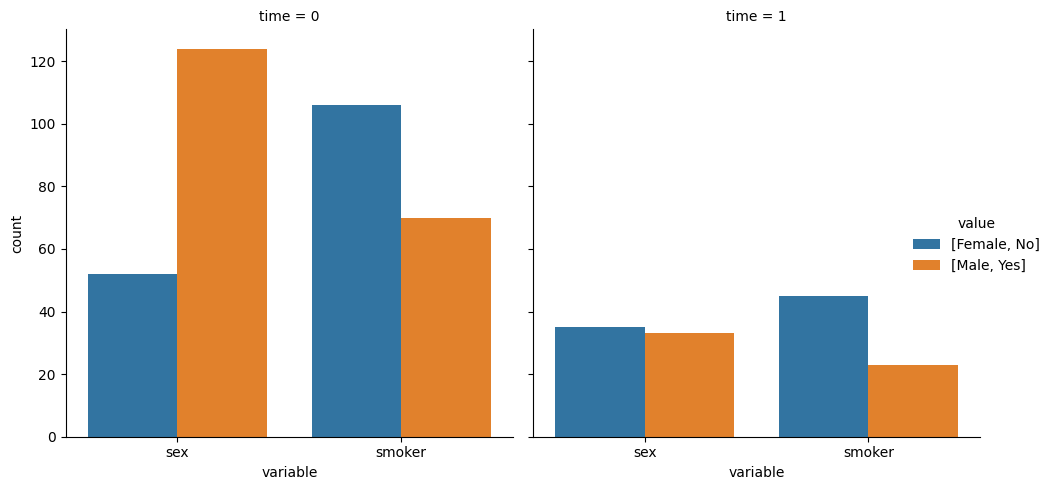
\includegraphics[width=0.8\textwidth]{img/catplot_5.png} 
    \caption{How combinations of smoker (smoker/non-smoker) and sex (gender) are distributed by time of day (lunch or dinner)}
    \label{fig:imagen}
\end{figure}

\section{References}

Waskom, M. L., (2021). seaborn: statistical data visualization. Journal of Open Source Software, 6(60), 3021, https://doi.org/10.21105/joss.03021.

\end{document}

